\documentclass[letterpaper,11pt]{book}
\usepackage[T1]{fontenc}
\usepackage[utf8]{inputenc}
\usepackage{lmodern}
\usepackage{float} % for floats other than tables and graphics
\usepackage[pdftex]{graphicx}

\setlength{\textwidth}{6.25in}
\setlength{\oddsidemargin}{0.25in}
\setlength{\evensidemargin}{0in}
\title{WBDC User's Guide}
\author{T. B. H. Kuiper}
\date{Revision of \today}

\floatstyle{boxed}
\newfloat{code}{h!tb}{cod}[chapter]
\floatname{code}{Snippet}

\begin{document}

\maketitle
\frontmatter
\chapter*{Preface}

Chapter~\ref{chap:intro}, Introduction, is a quick overview of WideBand 
DownConverter receiver class and its capabilities.

Chapter~\ref{chap:cmd-line}, Command Line, gives basic commands for direct 
control of the  equipment but also gives a simple, high-level view of the 
software organization.  

Chapter~\ref{chap:MandC}, Monitor and Control System, provides the details 
of the monitor and control system, such as component addresses and 
latch\footnote{A latch is an electronic logic device that retains the state
(0 or 1) assigned to it.} logic states.

Chapter~\ref{chap:config}, Configurations, explains how a WBDC is one element,
the {\tt Receiver}, in an over-all observing system.  Configurations describe 
how the signals flow between these elements.

A convention used in this document is that if an object is shown capitalized 
and in typewriter font, it is also a Python {\it class}\footnote{A class is a
programming unit that serves as a template for objects that are similar to
each other.  It has ``attributes'', such as
variables, and ``methods'' (functions). A class is a natural way of describing
a real-world object which has properties and can do things.}. In general,
a single word in typewriter font refers to an attribute while one followed by
empty parentheses is a method.

The most basic class is {\tt Device} which has the attributes 
{\tt name}, {\tt inputs} and {\tt outputs} which are instance of {\tt Port}
classes, and {\tt data} about the device, such as the location of a telescope
or the bandwidth of a receiver.  Most classes discused here are sub-classes of 
{\tt Device}, which means that they ``inherit'' these attributes.

In the hope that it is more enlightening than confusing, 
Snippet~\ref{code:classTelescope} (page~\pageref{code:classTelescope}) gives an
example of a class definition.
\begin{code}[h!tb]
\begin{center}
\begin{verbatim}
  
class Telescope(Device):
  def __init__(self, obs, dss=0, LO=None, active=True):
    name = "DSS-"+str(dss)
    Device.__init__(self, name)
    self.inputs = {obs.name:obs}
    self['longitude'], self['latitude'], self['elevation'], tz, name, diam = \
            get_geodetic_coords(dss=int(dss))
    self['geo-x'],self['geo-y'],self['geo-z'] = \
            get_cartesian_coordinates('DSS '+str(dss))
    self.outputs[self.name] = Port(self, self.name, signal=Beam(str(dss)))
    self.outputs[self.name].signal['dss'] = dss\end{verbatim}
\caption{\label{code:classTelescope}Stripped-down definition of the 
{\tt Telescope} class.}
\end{center}
\end{code}
The {\tt \_\_init\_\_()} method creates an instance of this class, which 
inherits attributes from the class {\tt Device}. The second line creates the 
object and the rest of the code assigns values to its attributes.

\tableofcontents
\listoffigures
\listof{code}{List of Code Examples}

\chapter*{Acronyms and Technical Terms}

\begin{description}\itemsep0pt \parskip0pt \parsep0pt
  \item[ADC]- analog-to-digital converter.
  \item[AIN]- LabJack\textsuperscript{\textregistered} analog input port.
  \item[DAC]- digital-to-analog converter.
  \item[DIO]- LabJack\textsuperscript{\textregistered} digital I/O.
  \item[IF]- intermediate frequency (signal) 
  \item[I/O]- input/output
  \item[I/Q]- in-phase/quadrature-phase, the two components of a complex signal.
  \item[K-band]- the frequency range 18-26.5~GHz.
  \item[LO]- local oscillator.
  \item[L/U]- lower sideband/upper sideband, a signal pair obtained from I/Q.
  \item[MSB]- most significant bit (or byte, depending on context).
  \item[PIN]- P-type/insulator/N-type, a type of diode.
  \item[RF]- radio frequency (signal)
  \item[WBDC]- wide-band down-converter, a class of receiver.
\end{description}

\mainmatter
\chapter{Introduction}\label{chap:intro}

\section{Hardware Overview}

A Wide-Band Down-Converter processes dual-polarization K-band signals from two
feed horns. There are two versions of the WBDC.  WBDC1 has two 
dual-polarization radio frequency sections after the band-splitting filters, one 
for 22 and 24~GHz, two switch-selectable local oscillators and one intermediate
frequency section. WBDC2 has five dual-polarization RF sections and 20 IF 
sections (2 feeds $\times$ 2 polarizations $\times$ 5 bands).

Figure~\ref{fig:inside} shows the interior of WBDC2.  The motherboard is on the
lid.   The RF enters through four SMA bulkhead feed-throughs on the left.  The
IFs exit on the right.

\begin{figure}[h!tb]
  \begin{center}
    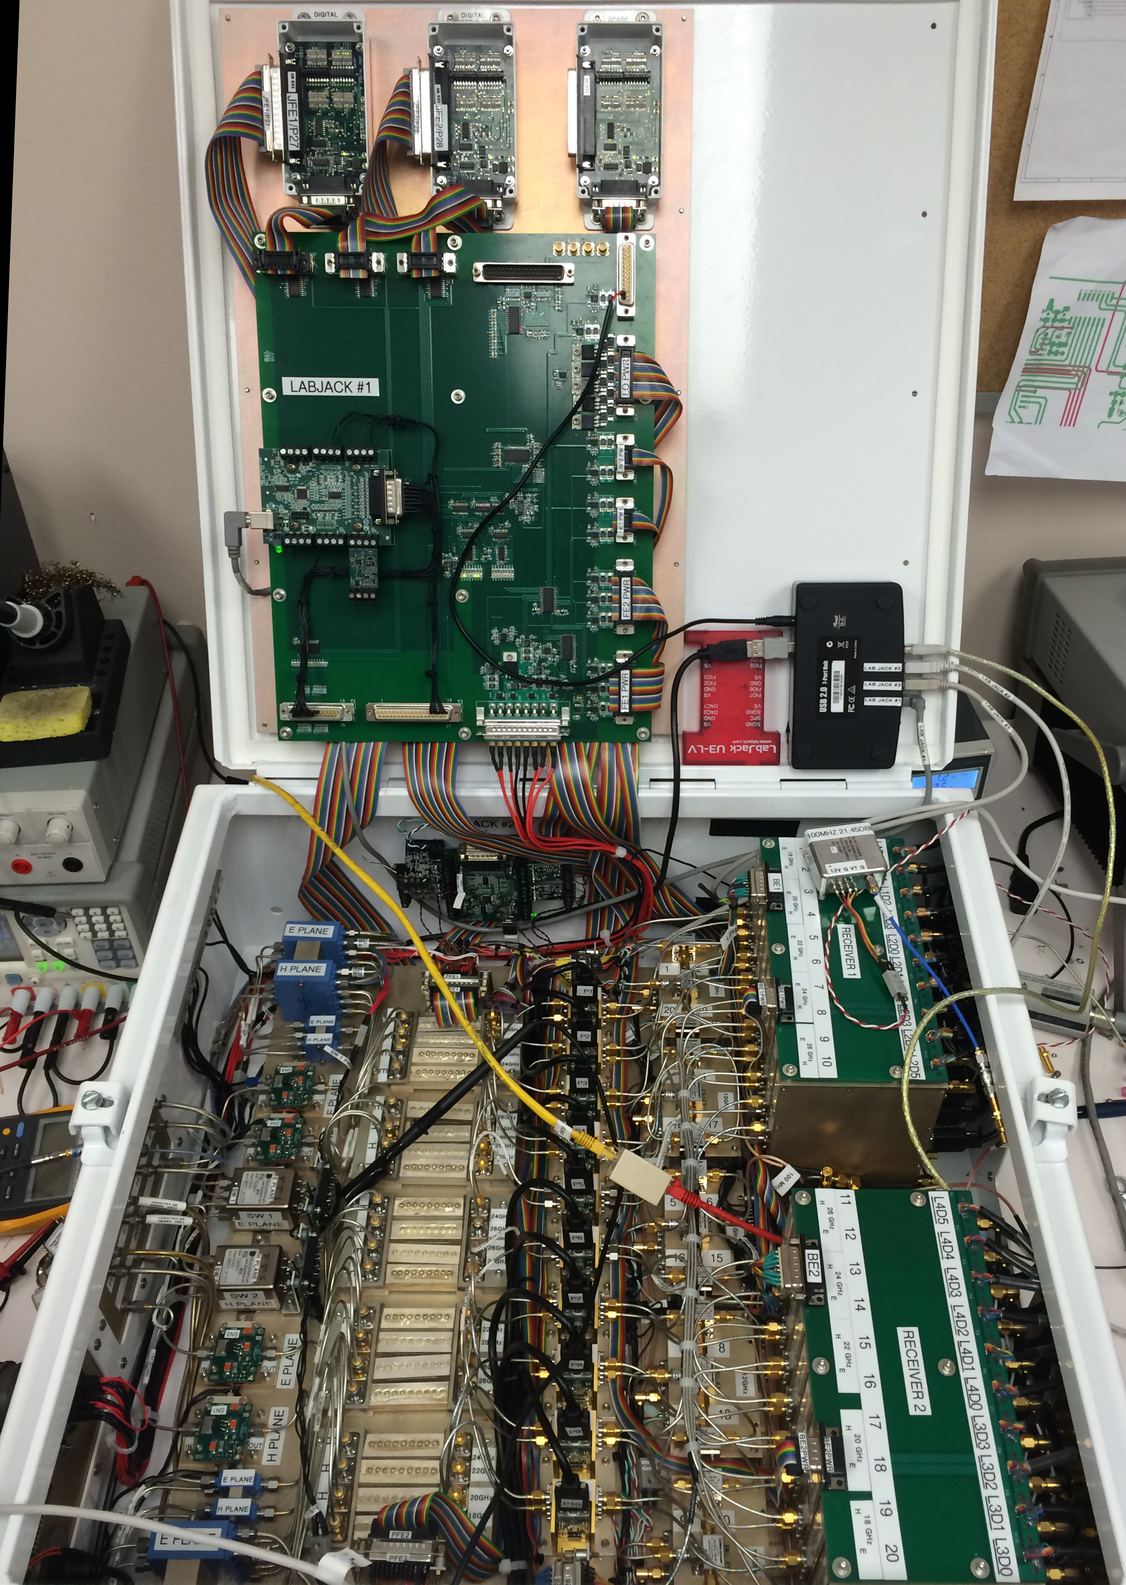
\includegraphics[height=5in]{interior-half.png}
  \end{center}
  \caption{\label{fig:inside}Interior of WBDC2.}
\end{figure}
The feed switching, polarization selection, and down-conversion are basically 
the same in both WBDC designs.  All functions are controlled by a motherboard
through LabJack\textsuperscript{\textregistered} general-purpose I/O 
interfaces.
The WBDC1 LabJacks are accessed through a USB hub by an external computer.  
WBDC2 LabJacks are controlled with a Raspberry Pi embedded computer accessed 
via ethernet.

\subsection{Input Switching}

The first stage of the WBDC allows the two dual-polarizationdown-converters to
be switched between the two feeds.  The switches are the two modules in the
center to the far left in Figure~\ref{fig:inside}.

\subsection{Polarization Conversion}

The four RF signals are split into five bands each. The splitters are the
larger blue modules at the top and bottom on the far left on 
Figure~\ref{fig:inside}.  After the band-selecting RF filters (row of modules 
to the left of center), the linearly polarized signals from each
feed can be switched into a quadrature hybrid (to the right of the black DB9
connectors) to be converted to circular
polarization.  PIN diode attenuators are provided (under the black
connectors) to balance the signals into
these hybrids.

\subsection{Sideband Separation}

In the closed modules on the far right are the down-converters, which have 
complex mixers putting out two IFs
from 0 to 1000~MHz, with a 90$^{\circ}$ phase difference.
Both IFs go from -1000~MHz to +1000~MHz but the negative and positive
frequencies are mixed together.
These may be considered the real and imaginary components of
a complex signal.
There are switches which can direct each I/Q pair into a quadrature
hybrid to convert them to an upper and lower sideband pair.

\section{Monitor and Control}

Monitor and control is done with two or three 
LabJack\textsuperscript{\textregistered} general purpose I/O devices. 

\subsection{LabJack 1}

This LabJack with local ID 1 (on the center left of the motherboard) controls 
the WBDC motherboard.   The motherboard has groups of
eight latches which are used to control and sense switches, and to select
analog monitoring points.  The LabJack's ADC channels read currents, voltages, 
and temperatures. 

\subsection{Labjack 2 (and 3)}

LabJack 2 (and 3 for WBDC2), on the box walls at the ends of the row of 
filters, control PIN diode attenuators.
There are four voltage-controlled RF attenuators (PIN diodes) for each
down-converter sub-band.  The voltages are generated in LabJack
TickDACs attached to the terminals of LabJack 2 (and 3 for WBDC2).


\chapter{Command Line}\label{chap:cmd-line}

The program {\tt wbdc2\_prompt.py}\footnote{In
{\scriptsize \tt /usr/local/lib/python2.7/DSN-Sci-packages/MonitorControl/Receivers/WBDC/apps}.}
provides the user with a direct Python command line interface in a terminal 
session on the embedded Raspberry Pi.  It simply configures the hardware and 
software as described in Chapter~\ref{chap:config}.

The programming style used is ``object oriented'', so that a command takes the 
form {\tt object.method()} where {\tt object} is an ``instance'' of a ``class'.
In this implementation, classes may have private classes. Think of systems and 
subsystems, so that a command can also have the form
{\tt parent.child.method()}. Classes can also have instances of other public
classes as ``attributes'', which leads to the same command structure.
In the program {\tt wbdc2\_prompt.py}, {\tt receiver} is an instance of the
{\tt WBDC2} class.

The Python {\tt help()} command can be very useful at the command line.  It can
be invoked at any level of the hierarchy.  These examples 
\begin{verbatim}
  help(receiver)
  help(receiver.get_crossover)
  help(receiver.crossSwitch)
  help(receiver.crossSwitch.get_state)\end{verbatim}
will become clearer below.

\section{High-level Commands}

\subsection{Feed Switch Control}\label{subsec:feed_switch}

The WBDC class of receivers have two feed horns with two linear polarizations,
``E'' and ``H''.  There are four input channels called ``F1E'', ``F1H'',
``F2E'' and ``F2H''.  These feed a pair of switches through which the receivers
connect to the feeds.  In the default state (logic state 0),
``F1E''$\rightarrow$``R1E'' and ``F1H''$\rightarrow$``R1H''.  In the {\it set}
state (logic state 1), ``F1E''$\rightarrow$``R2E'' and 
``F1H''$\rightarrow$``R2H''.  The commands for this are shown in 
Snippet~\ref{code:crossover}.
\begin{code}[h!tb]
\begin{center}
  \begin{verbatim}
  
  receiver.get_crossover()
  receiver.set_crossover(crossover=False)\end{verbatim}
\caption{\label{code:crossover}Sensing and controlling the transfer switch.}
\end{center}
\end{code}
The keyword {\tt crossover} is not required in this case but is
mnemonically useful. The value {\tt True} sets the switch.

\subsection{Polarization Mode}

Each of the four receiver sections feeds five bandpass filters.
``Band 18'' goes from 17 to 19~GHz, ``Band 20'' from 19 to 21, and so on to
``Band 26'' from 25 to 27 GHz.  There are ten sections which can convert the
linearly polarized modes ``E'' and ``H'' produced by the front end to 
circularly polarized modes ``L'' and ``R''.  

The command for sensing and controlling the polarization mode are given in
Snippet~\ref{code:polsec}.
\begin{code}[h!tb]
\begin{center}
  \begin{verbatim}
  
  receiver.get_pol_modes()
  receiver.set_pol_modes(circular=False)\end{verbatim}
\caption{\label{code:polsec}Sensing and controlling the polarization mode.}
\end{center}
\end{code}
{\tt receiver.get\_pol\_modes()} returns a Python {\tt dict} (short for 
``dictionary'') which is a key:value  array with the states of all the 
polarization sections.  The command {\tt receiver.set\_pol\_modes()}
sets all the polarization sections in the entire receiver to the designated
state. The default state, that is, if {\tt set\_pol\_modes()} is invoked
without specifying an argument, is {\tt False}.  This command automatically 
invokes {\tt get\_pol\_modes()} as its last step.

\subsection{Down-conversion Mode}

The outputs from the polarization sections go into down-converters which have
names like ``DC['R1-18P1']'' (receiver 1, band 18, polarization 1) which 
reflects the fact that the polarization is
now ambiguous. ``P1'' can be ``E'' or ``L'' while ``P2'' can be ``H'' or ``R''
depending on the state of the polarization section providing the signal.

There are quadrature hybrids which may be used to convert the
in-phase and quad-phase IFs to lower sideband (-1000 to 0~MHz) and upper 
sideband (0 to 1000~MHz) IFs.  The default state (logic 0) of these sections is
L/U mode; the optional I/Q mode is logic state 1.  

The commands for sensing and controlling the down-converter section IF mode is
shown in Snippet~\ref{code:DCsec}.
\begin{code}[h!tb]
\begin{center}
  \begin{verbatim}
  
  receiver.get_IF_mode()
  set_IF_mode(SB_separated=False)\end{verbatim}
\caption{\label{code:DCsec}Sensing and controlling the down-converter mode.}
\end{center}
\end{code}
The first command
returns a Python {\tt dict} with the states of all the downconverters.
All the downconverters can be set to the same state with the command
{\tt set\_IF\_mode()}.
It also returns a Python {\tt dict} with the states of all the downconverters.

\subsection{Analog Monitoring}

The analog inputs to LabJack 1 are connected to various analog monitoring
points.
The power supply voltages, currents to various subsystems, temperatures at
three locations and the power levels into the RF sections can all be monitored.

Analog inputs 0 and 1 return currents and voltages respectively. AIN2 and AIN3 
return RF power and temperature. The address of the current and voltage monitor
point is sent to latchgroup 1 at address 0.  The address of the RF power and
temperature is sent to latchgroup 1 at address 2.

The command {\tt receiver.readAnalogs(latchAddress)} returns a Python dict with
all the analog data available through that latch group.

\subsection{Other}

For completeness we note here one other high-level command which can be useful
for debugging the equipment.
\begin{verbatim}
  receiver.check_IO_config()
\end{verbatim}
reports on the configuration of the WBDC2's three LabJack multi-purpose I/O
devices. Section~\ref{sec:cfg_chk} shows a typical output and the proper
configuration of the LabJacks.


\section{Mid-level Commands}

\subsection{Feed Switch Control}

The crossover switch subsystem can be addressed directly.
The commands to check and set the state of the cross-over switch are shown in
Snippet~\ref{code:Xswitch}.
\begin{code}[h!tb]
\begin{center}
  \begin{verbatim}

  receiver.crossSwitch.get_state()
  receiver.crossSwitch.set_state(True)\end{verbatim}
  \caption{\label{code:Xswitch}Sensing and controlling the crossover switch
directly.}
\end{center}
\end{code}
These have the same effect as the commands shown in 
Snippet~\ref{code:crossover}.


It can happen that the two switches are not in the same state.  Then
{\tt get\_crossover()} will give an error message.  The state of the individual
switches can be queried with the commands in Snippet~\ref{code:xswitch}.
\begin{code}[h!tb]
\begin{center}
  \begin{verbatim}
  
  receiver.crossSwitch['E'].get_state()
  receiver.crossSwitch['H'].get_state()\end{verbatim}
  \caption{\label{code:xswitch}Sensing the state of the individual crossover
  switches.}
\end{center}
\end{code}
The switches can be set individually with similar {\tt set\_state()} commands.

\subsection{Polarization Mode}

The state of the individual polarization sections can be queried and set with
the commands in Snippet~\ref{code:pol_sec}.
\begin{code}[h!tb]
\begin{center}
\begin{verbatim}

  receiver.pol_sec['R120'].get_state()
  receiver.pol_sec['R120'].set_state(True)
  receiver.pol_sec['R1-18'].atten['H'].set_atten(10)\end{verbatim}
  \caption[Control of individual polarization sections]
  {\label{code:pol_sec}Commands
  to sense and set the mode of individual
  polarization sections and to balance their inputs.}
\end{center}
\end{code}  
The {\it set} state (logic level 1) means that the conversion is made.  The
default state is {\tt False} (logic level 0).
For the polarization sections to function properly, the two incoming signals
must be balanced.  For that purpose, each polarization section has two
attenuators which can be adjusted.  (The balancing procedure is described
elsewhere.) 
The attenuation can be queried with a corresponding {\tt get\_atten()}
command but it does not read the hardware.  It only reports what the last
{\tt set\_atten()} command did.  The attenuation specified is relative to
the minimum attenuation of the attenuator, which is in the range of 7 to 9~dB.

The state of a single down-converter hybrid can be queried and set
with commands like those in Snippet~\ref{code:IQhybrids}.
\begin{code}[h!tb]
\begin{center}
\begin{verbatim}

  receiver.DC['R1-18P1'].get_state()
  receiver.DC['R1-18P1'].set_state(True)\end{verbatim}
\caption{\label{code:IQhybrids}Commands for sensing and setting a 
down-converter I/Q hybrid.}
\end{center}
\end{code}



\section{Low Level Commands}

\subsection{LabJacks}

At the heart of the monitor and control subsystem are two (or three) 
LabJacks.  (They can also provide other functions, like timers,
which we don't use.)

There are eight I/O lines available at screw terminals on the unit. These can
all function as digital inputs or outputs, or analog inputs, according to the
value of some configuration bytes.  They are called FIO0-FIO7 when functioning
as digital ports and AIN0-AIN7 when functioning as analog ports.  In addition,
the DB25 connector on the LabJacks provides an additional 12 digital IO lines,
called EIO0-EIO7 and CIO0-CIO3.  Each LabJack also has two analog
outputs called DAC0 and DAC1, which we don't use.

Communication with the LabJack consists mainly of reading and writing bytes to
the FIO, DIO and CIO groups.


\subsection{Digital Monitor and Control}

All the switches described above are controlled by latches.  The latches are
logically grouped, as shown in Table~\ref{tab:latches}, with up to eight
latches per group.
\begin{table}[h!tb]
  \begin{center}
    \caption{\label{tab:latches}Latch Groups for Digital Monitor and Control}
    \begin{tabular}{|c|l|}
      \hline
      {\bf Latch Group} & {\bf Function} \\
      \hline
      X & controls the cross-over switches \\
      R1P & controls the receiver 1 polarization sections \\
      R2P & controls the receiver 1 polarization sections \\
      PLL & monitors the cross-over switch state and LO phase lock \\
      P1I1 & pol 1 IF group 1 (bands 18 and 20) \\
      P1I2 & pol 1 IF group 2 (bands 22, 24 and 26) \\
      P2I1 & pol 2 IF group 1 (bands 18 and 20) \\
      P2I2 & pol 2 IF group 2 (bands 22, 24 and 26) \\
      \hline
    \end{tabular}
  \end{center}
\end{table}
Latch groups are read as bytes, as shown by the examples in 
Snippet~\ref{code:LGm&c}.
\begin{code}[h!tb]
\begin{center}
\begin{verbatim}

  In [7]: Math.decimal_to_binary(receiver.lg['P2I2'].read())
  Out[7]: '00000000'
  In [12]: Math.decimal_to_binary(receiver.lg['PLL'].read())
  Out[12]: '01110100'
\end{verbatim}
\caption{\label{code:LGm&c}Setting a latch group.}
\end{center}
\end{code}
The bit assignment for each latch group is described in
Subsection~\ref{subsec:DM1}.  There is a
corresponding {\tt write()} command which could be used in this way
\begin{verbatim}
  receiver.lg['X'].write(int('00000011',2))
\end{verbatim}
to set the cross-over switches.

\subsection{Attenuator Control}

The attenuators are PIN diodes
controlled with a voltage (or more strictly, the current resulting from an
applied voltage).  The voltages are supplied by dual-channel (``A'' and
``B'') digital-to-analog converters.  The DACs are connected to a LabJack
multi-function IO interface.

In the example in Snippet~\ref{code:DAC}
an instance of a DAC is created and the A side is set to -2~V.
\begin{code}[h!tb]
\begin{center}
\begin{verbatim}

  from Receiver.Interfaces.LabJack import LJTickDAC
  
  LJTickDAC(receiver.LJ[2],'R1-18')['A'].setVoltage(-2)
  
  vs = LJTickDAC(receiver.LJ[2],'R1-18')['A']
  vs.setVoltage(-2)\end{verbatim}
\caption{\label{code:DAC}Two ways of instantiating and setting a DAC.}  
\end{center}
\end{code}
The first way avoids creating an enduring instance of the DAC.  However, it is
pretty cumbersome so the second way, which creates an instance of a DAC,
although taking two steps, is usually preferred.  And there might be need to
use {\tt vs} again.

The LJTickDAC is an ``attribute'' of the polarization section and so also be 
addressed as {\tt receiver.pol\_sec['R1-18'].tdac['A']}.

Using this command to control the attenuation requires knowledge of the 
attenuation {\it vs} control voltage curve.  This is discussed elsewhere.


\chapter{Monitor and Control System}\label{chap:MandC}

\section{Motherboard Control}

Motherboard signals are monitored and controlled with digital latches (logical
devices which preserve a specified logic state). The latches are connected to
serial-in/parallel-out registers.  These registers are addressed using the EIO
out bits of LabJack 1.  The data are then clocked into the register using
the SDI and SCK signals.  Table~\ref{tab:signals} shows how the LabJack ports 
are used to control the motherboard signals.
\begin{table}[h!tb]
  \begin{center}
    \caption{\label{tab:signals}Motherboard Signals and LabJack Ports}
    \begin{tabular}{|c|r|l|l|}
    \hline
    \multicolumn{2}{|c|}{\bf Labjack} & \multicolumn{2}{c|}{\bf WBDC Motherboard} \\
    \hline
     {\bf Name} & {\bf Channel} & {\bf Name}  & {\bf Function} \\
    \hline
      AIN0  &   0    & IMON &  Analog input measuring supply currents \\
      AIN1  &   1    & VMON &  Analog Input measuring supply voltages \\
      AIN2  &   2    & TEMP &  Analog input measuring temperatures \\
      AIN3  &   3    & RF   &  Analog input measuring RF power \\
      FI04  &   4    &      & \\
      FI05  &   5    &      & \\
      FI06  &   6    &      & \\
      FI07  &   7    & SDO  &  Digital input from readback \\
   \hline
      EI00  &   8    & A0   &      Latch address LSB \\
      EI01  &   9    & A1   &      .. \\
      EI02  &  10    & A2   &      .. \\
      EI03  &  11    & A3   &      .. \\
      EI04  &  12    & A4   &      .. \\
      EI05  &  13    & A5   &      .. \\
      EI06  &  14    & A6   &      .. \\
      EI07  &  15    & A7   &      Latch address MSB \\
    \hline
      CI00  &  16    & SCK     &   Serial Clock input \\
      CI01  &  17    & SDI     &   Data input \\
      CI02  &  18    & NLOAD   &   Load data to/from latches \\
      CI03  &  19    & CS-BUS  &   Eable writing to or reading from latch \\
    \hline  
    \end{tabular}
  \end{center}
\end{table}
The state of NLOAD is normallly high. When checking status (or reading bits),
NLOAD is toggled low for at least 10 mS then high to store the information for
reading.
CS-BUS is the global enable. The normal state is high. This is set to low when
programming latches or reading data. It is set high when done.

LabJack 1 is capable of addressing 256 latches on a WBDC motherboard.
They are grouped in 32 sets of 8 latches. The first four of the latch groups,
at addresses 0--3, 8--11, 16--19, ..., 80--83, ..., 248--251,
are writing to control bits. The second four of the latch group,
at addresses 4--7, 12--15, 20--23, ...,84--87, ..., 252--255,
are for reading from control or status bits ({\it e.g.} switch position 
indicators).

Latch group address bits A0-A7 (ports EIO0--EIO7 on LabJack 1) are used to 
address a specific 8-bit latch group for writing or reading. The latch data are
bytes sent or read serially, MSB first.  The latch group address encoded with 
the EIO bits consists of three parts:
\begin{description}\itemsep0pt \parskip0pt \parsep0pt
  \item[EIO7-EIO3]  encodes the motherboard digital module (DM = 1, 2, or 3) 
  address.
  \item[EIO2] indicates write if 0 and read if 1.
  \item[EIO1-EIO0] along with EIO2, selects the latch group (LG = 1-4) in a 
  digital  module.
\end{description}
So latches in write-mode have addresses ending in 0--3.  Latches in read-mode
have addresses ending in 4--7. 

The DM 1 bit address assignment differs for 
WBDC1 and WBDC2. DM~1 LG~1 has a EIO value (address) of 80 (0101~0000) in WBDC1
and 8 (0000~1000) in WBDC2. LG~2 in any DM has EIO0=1.   WBDC2 DM~2 LG~1 has 
address 16 (0001~0000).



\subsection{Digital Module 1}\label{subsec:DM1}

Seven latch groups are assigned to digital monitoring, that is, the program
reads the latch states.

\subsubsection{Feed Crossover Switch}

The feed crossover switches are controlled with DM 1 LG 1 using bits L1A0 and
L1A1 (A0, A1 on latchgroup 1): logic~0 for through and logic~1 for 
crossed. The commanded state can be read at the same bits (A0, A1 at LG address
12). However, the actual states of the cross-over switches are read at L4A0 and
L4A1 (LG 3).

\subsubsection{Polarization Hybrids}

\paragraph{WBDC1} (to be provided).

\paragraph{WBDC2} receiver chain~1 polarization hybrids are controlled by
latchgroups 2 and 3. 
The receiver chain~1 polarization hybrids are controlled by L2A0--L2A4.
The receiver chain~2 polarization hybrids are controlled by L3A0--L3A4.
\begin{verbatim}
  Band  Control Bits
   18    L2A0 L3A0
   20    L2A1 L3A1
   22    L2A2 L3A2
   24    L2A3 L3A3
   26    L2A4 L3A4
 \end{verbatim}
 Logic level~0 is for bypassing the hybrids, that is, linear polarization.
Logic level~1 is for converting linear to circular, that is, X and Y
polarization to L and R.


\subsubsection{Local Oscillator Lock}

Latch Group 4 monitors the state of the transfer switches and the local 
oscillator phase-locked loops
\begin{verbatim}
  Pol   Status Bit
    X      L4A0
    Y      L4A1
  Band  Status Bit
   18      L4A2
   20      L4A3
   22      L4A4
   24      L4A5
   26      L4A6 
\end{verbatim}

\subsubsection{Latch LEDs}

The monitor bits should match the LEDs in the respective digital module.
In WBDC1 the DM is to the top right
With the hinge of the lid at the bottom, the LabJacks are upside down. 
The LEDs are in LSB -> MSB order and grouped as
\begin{verbatim}
LG 3 address 82 or 86    LG 4 address 83 or 87
LG 1 address 80 or 84    LG 2 address 81 or 85
\end{verbatim}
If the box is mounted on a wall or ceiling and the lid is hanging down,
the order is more conventional.

In WBDC2 there are three DMs at the top left of the lids, numbered from left
to right.  DM~3 is a spare. The (upside down) LED ordering is
\begin{verbatim}
LG addr 10 or 14   LG addr 11 or 15         LG addr 18 or 22   LG addr 19 or 23
LG addr  8 or 12   LG addr  9 or 13         LG addr 16 or 20   LG addr 17 or 21
\end{verbatim}

\subsection{Digital Module 2}

This only applies to WBDC2.  Four latch groups are used to control the I/Q
hybrids.
Receiver chain 1 I/Q hybrids are controlled by latch groups 1 and~2 (low 
address). Receiver chain 2 I/Q hybrids are controlled by latch groups 3 and~4
(low address).
The two bypass switches for each hybrid are controlled with one bit.
Logic level 1 is for IQ; logic level 0 is for LU.
This is the bit assigment:
\begin{verbatim}
          Pol 1        Pol 2
  Band  Rec1  Rec2   Rec1  Rec2
   18   L1A0  L1A1   L3A0  L3A1
   20   L1A2  L1A3   L3A2  L3A3
   22   L2A0  L2A1   L4A0  L4A1
   24   L2A2  L2A3   L4A1  L4A2
   26   L2A4  L2A5   L4A3  L4A4
\end{verbatim}
   
\subsection{WBDC1 Analog Monitoring}

Latch addresses 0 and 2 address the
registers used to select analog monitoring points.
bit pattern sent to latch address 0 selects a current and a voltage
to be connected to AIN0 and AIN1.  A bit pattern sent to latch address
2 selects a thermistor to be connected to AIN2.  AIN3 is not used in this
receiver.

(Register addresses to be provided.)

\subsection{WBDC2 Analog Monitoring}

\subsubsection{Latch 1 (Address 0)}

This latch addresses the register used to select voltage and current monitoring
points.  Voltage points are
selected using bits 0-2 and read at AIN1.  Currents are selected using bits
3-6 and read at AIN0.  The addresses can be ANDed to select any voltage point
with any current point.  

The monitor point address bits for voltage are shown in Table~\ref{tab:volt-mon}. 
The actual voltages are the byte read times the scale factor shown in 
Table~\ref{tab:volt-mon}
\begin{table}[h!tb]
  \begin{center}
    \caption{\label{tab:volt-mon}Monitor Points for Voltages}
    \begin{tabular}{|c|c|c|rl|r|}
    \hline
\multicolumn{2}{|c|}{\bf Latch} & \multicolumn{4}{c|}{ } \\ 
\hline  
{\bf Address} & {\bf Bits}      & {\bf Input}  & \multicolumn{2}{c|}{\bf Supply }  & {\bf Scale} \\
\hline
0       & {\tt xxxxx000}  & AIN1 &  +6 V & digital        &   4.0211 \\
0       & {\tt xxxxx001}  & AIN1 &  +6 V & analog         &   4.0278 \\
0       & {\tt xxxxx010}  & AIN1 & +16 V &                &  10.5446 \\
0       & {\tt xxxxx011}  & AIN1 & +12 V &                &  10.5827 \\
0       & {\tt xxxxx100}  & AIN1 & -16 V &                & -10.5446 \\
\hline
    \end{tabular}
  \end{center}
\end{table}

The monitor point addresses for currents are shown in 
Table~\ref{tab:I-mon-points}.
The actual currents are the value read offset by -0.026.
\begin{table}[h!tb]
  \begin{center}
    \caption{\label{tab:I-mon-points}Monitor Points for Currents}
    \begin{tabular}{|c|c|c|rl|}
    \hline
\multicolumn{2}{|c|}{\bf Latch} & \multicolumn{3}{c|}{ } \\ 
\hline  
{\bf Address} & {\bf Bits} & {\bf Input} & \multicolumn{2}{c}{\bf Supply }  \\
\hline
0 & {\tt x0000xxx} & AIN0 & +6 V  & MB digital  \\
0 & {\tt x0001xxx} & AIN0 & +6 V  & MB analog   \\
0 & {\tt x0010xxx} & AIN0 & -16 V & MB          \\
0 & {\tt x0011xxx} & AIN0 & +16 V & R1 FE  \\
0 & {\tt x0100xxx} & AIN0 & +16 V & R2 FE  \\
0 & {\tt x0101xxx} & AIN0 & +16 V & R1 BE  \\
0 & {\tt x0110xxx} & AIN0 & +16 V & R2 BE  \\
0 & {\tt x0111xxx} & AIN0 & +16 V & LDROs  \\
0 & {\tt x1000xxx} & AIN0 & +16 V & MB     \\
0 & {\tt x1001xxx} & AIN0 &  +6 V & R1 FE  \\
0 & {\tt x1010xxx} & AIN0 &  +6 V & R2 FE  \\
0 & {\tt x1011xxx} & AIN0 & -16 V & R1 FE  \\
0 & {\tt x1100xxx} & AIN0 & -16 V & R2 FE \\
0 & {\tt x1101xxx} & AIN0 & -16 V & R1 BE  \\
0 & {\tt x1110xxx} & AIN0 & -16 V & R2 BE  \\
\hline
    \end{tabular}
  \end{center}
\end{table}


\subsubsection{Latch 2 (Address 1)}

This latch selects temperature monitor point with bits 0--2 to be read at AIN3
and RF detector voltages with bits 3--6 to be read at AIN2.
Table~\ref{tab:T-mon-points} gives the monitor address bits for temperature.
\begin{table}[h!tb]
  \begin{center}
    \caption{\label{tab:T-mon-points}Monitor Points for Temperatures}
    \small \begin{tabular}{|c|c|c|rl|}
\hline  
{\bf Address} & {\bf Bits} & {\bf Input} & {\bf Supply |} & {\bf Location}  \\
\hline
1 & {\tt xxxxx000} & AIN3 & & R1 RF plate  \\
1 & {\tt xxxxx001} & AIN3 & & R2 RF plate  \\
1 & {\tt xxxxx010} & AIN3 & & BE plate     \\
 \hline
    \end{tabular}
  \end{center}
\end{table}
The conversion from measured volts to temperature is
\begin{displaymath}
  T = (V_{AIN3}+0.2389275)*23.549481
\end{displaymath}

The monitor points for RF detector power are given by 
Table~\ref{tab:RF-mon-points}.
\begin{table}[h!tb]
  \begin{center}
    \caption{\label{tab:RF-mon-points}Monitor Points for RF Detectors}
    \small \begin{tabular}{|c|c|c|c|}
     \hline
{\bf Address} & {\bf Bits}     & {\bf Input} & {\bf Location}  \\
\hline
1             & {\tt x0000xxx} & AIN2        & R1 E-plane  \\
1             & {\tt x0001xxx} & AIN2        & R2 E-plane  \\
1             & {\tt x0010xxx} & AIN2        & R1 H-plane \\
1             & {\tt x0011xxx} & AIN2        & R2 H-plane  \\
 \hline
    \end{tabular}
  \end{center}
\end{table}
The actual reading is (data-0.004)*2.0064.

\chapter{Configurations}\label{chap:config}

A WBDC is one element of a receiving system, specifically a {\tt Receiver}.  The
receiver obtains its signals from a front end and delivers signals to a 
backend.  A configuration is a description of the signal flow from the point
where the antenna focuses radiation on a feed to the point where data are
processed by a computer.  At the very minimum, a receiver must know something
about where its signal comes from and what properties were imposed by the
preceding equipment.

Configurations are stored in the {\tt DSN-Sci-packages} directory under\linebreak
{\tt MonitorControl/Configurations}.  The configuration used by the 
program {\tt wbdc2\_prompt.py} is shown in Snippet~\ref{code:config}.
\begin{code}[h!tb]
\begin{center}
\begin{verbatim}

from MonitorControl import Observatory, Telescope, ClassInstance
from MonitorControl.FrontEnds import FrontEnd
from MonitorControl.FrontEnds.K_band import K_4ch
from MonitorControl.Receivers import Receiver
from MonitorControl.Receivers.WBDC.WBDC2 import WBDC2

import logging
module_logger = logging.getLogger(__name__)

def station_configuration(roach_loglevel=logging.WARNING):
  """
  Configuration for the K-band system on DSS-43 using WBDC2

  Feed 1 (F1) is at 024-0.016, F2 at 024+0.016.  The polarizations are linear,
  E and H.  There are so many receiver outputs that it is simpler to let the
  software generate them.
  """
  observatory = Observatory("Canberra")
  telescope = Telescope(observatory, dss=43)
  front_end = ClassInstance(FrontEnd, K_4ch, "K",
                     inputs = {'KF1': telescope.outputs[telescope.name],
                               'KF2': telescope.outputs[telescope.name]},
                     output_names = [['F1E','F1H'],
                                     ['F2E','F2H']])
  IFswitch = None
  receiver = ClassInstance(Receiver, WBDC2, "WBDC-2",
                           inputs = {'F1E': front_end.outputs["F1E"],
                                     'F1H': front_end.outputs["F1H"],
                                     'F2E': front_end.outputs["F2E"],
                                     'F2H': front_end.outputs["F2H"]})
  clock = None
  backend = None
  return observatory, telescope, front_end, receiver, IFswitch, clock, backend\end{verbatim}
\caption[Configuration used by {\tt wbdc2\_prompt.py}]{\label{code:config}
Configuration description used by the program
{\tt wbdc2\_prompt.py} to test WBDC2 in the lab.}
\end{center}
\end{code}
This shows that the {\tt Receiver} is a class {\tt WBDC2} device with the name
``WBDC2''.  It has four inputs named ``F1E'', ``F1H'', ``F2E'' and
``F2H'' which were introduced in Subsection~\ref{subsec:feed_switch}. They
obtain their signals from front end outputs with the same names.  They
don't have to be the same but it was natural in this case.  In general, port
names can be the label for the port on the device.

In this case the description stops at the WBDC.  However, a phantom 
{\tt FrontEnd} object (one that can't be controlled or monitored) had to be 
defined because the {\tt Receiver} expects a signal source.  The 
{\tt FrontEnd} needs a {\tt Telescope} for a signal.

The {\tt Observatory} provides a context for the {\tt Telescope}.  There are
devices which depend on the observatory, rather than a particular telescope.
The {\tt Telescope} object has one output which provides the signal to one or
more input ports of the {\tt FrontEnd}.  The {\tt Observatory} object has
information not specific to a {\tt Telescope}, such as weather data.


\appendix
\chapter{LabJack Configuration}

\section{LabJack 1}

This monitors and controls the motherboard.
\begin{verbatim}
  FIO0-FIO3 - AIN: monitor voltages, current, temperatures
  FIO4-FIO6 -      not used
  FIO7      - DO:  read digital in
  EIO0-EIO7 - DO:  select latch by address
  CIO0-CIO3 - DO:  set WBDC signals
\end{verbatim}
So this is the LabJack Configuration
\begin{verbatim}
              CIOBitDir     1111
              EIOBitDir 11111111
              FIOBitDir 00000000
              FIOAnalog 00001111
\end{verbatim}

\section{LabJack 2 (and 3)}

This controls the LJTickDAC\textsuperscript{\textregistered} voltage sources.
All EIO and CIO ports are assigned to controlling this function and so are
digital outputs.

\section{Configuration Check}\label{sec:cfg_chk}

An initial checkout might be as shown in Snippet~\ref{code:cfg_chk}.
\begin{code}[h!tb]
\begin{center}
\begin{verbatim}

  In [2]: from MonitorControl.Electronic.Interfaces.LabJack import *
  In [3]: lj = connect_to_U3s()
  In [4]: report_IO_config(lj)\end{verbatim}
\caption{\label{code:cfg_chk}Commands for checking the LabJack I/O
configuration.}
\end{center}
\end{code}
The normal state of the WBDC1 LabJacks is something like
\begin{verbatim}
=============== U3 I/O Configurations ================
          U3 local ID          1        2
          ------------- -------- --------
              CIOBitDir 00001111 00000000
               CIOState 00001111 00001111
             DAC1Enable 00000000 00000000
              EIOAnalog 00000000 00000000
               EIOState 01010111 11111111
         EnableCounter0    0.000    0.000
         EnableCounter1    0.000    0.000
                  FAIN0    0.001
                  FAIN1    1.455
                  FAIN2    0.000
                  FAIN3    0.000
              FIOAnalog 00001111 00000000
              FIOBitDir 00000000 00000000
               FIOState 11110000 11111111
  NumberOfTimersEnabled        0        0
          Temperature  295.569  295.507
     TimerCounterConfig       64       64
  TimerCounterPinOffset        4        4
\end{verbatim}

\end{document}
